% Esqueleto do artigo. Troque o preâmbulo pelo do template OFICIAL que o professor indicar (SBC ou IEEE).
% No template SBC o preâmbulo é: \documentclass[12pt]{article} \usepackage{sbc-template}
% (sbc-template.sty é baixado do site da SBC; coloque-o nesta pasta e descomente a linha abaixo.)
% Marcadores: \todo{...} = falta escrever; [A]/[B]/[C]/[D] = pessoa dona da seção.
\documentclass[12pt]{article}
% \usepackage{sbc-template}
\usepackage[margin=2.5cm]{geometry}   % remova ao usar o sbc-template
\usepackage{graphicx,url,booktabs}
\usepackage[brazilian]{babel}
\usepackage[utf8]{inputenc}
\usepackage[T1]{fontenc}
\newcommand{\todo}[1]{\textbf{[TODO: #1]}}

\title{GraphRAG para História da Computação: grafo de conhecimento em Neo4j para reduzir alucinações em perguntas multi-hop}
\author{Nome 1, Nome 2, Nome 3, Nome 4 \\ Instituição \\ \texttt{emails}}
\date{}

\begin{document}
\maketitle

\begin{abstract}
\todo{[D, escrever por último] 150--200 palavras: problema (alucinação e perguntas que exigem vários saltos),
abordagem (extração de grafo + Neo4j + recuperação híbrida), experimento (RAG vetorial puro $\times$ GraphRAG em
\emph{N} perguntas) e o principal resultado numérico.}
\end{abstract}

\section{Introdução} % [D]
\todo{Motivação: LLMs alucinam; RAG vetorial recupera trechos parecidos, mas falha quando a resposta exige
ligar fatos de documentos diferentes (multi-hop).}
\todo{Pergunta de pesquisa: um grafo de conhecimento em Neo4j, combinado com busca vetorial, reduz alucinações e
melhora respostas multi-hop frente ao RAG vetorial puro?}
\todo{Contribuições (3 itens): pipeline texto$\to$grafo; recuperação híbrida com text-to-Cypher e algoritmos de grafo;
avaliação comparativa com métrica de alucinação.}
\todo{Organização do artigo.}

\section{Fundamentação e trabalhos relacionados} % [D]
\todo{RAG~\cite{lewis2020rag}; GraphRAG~\cite{edge2024graphrag}; KAG~\cite{liang2024kag};
bancos de grafos e Cypher~\cite{robinson2015graph,francis2018cypher}; PageRank~\cite{page1999pagerank} e
Louvain~\cite{blondel2008louvain}; embeddings~\cite{reimers2019sbert}.}
\todo{Uma tabela curta comparando as abordagens (o que recupera, como cita a fonte, limitação).}

\section{Domínio e dados} % [A]
Domínio: História da Computação, a partir de páginas da Wikipédia em português.
O grafo final tem 27 documentos, 86 \emph{chunks}, 637 entidades e 364 relações
(\todo{conferir números na versão final do \texttt{grafo.json}}).
\todo{Por que esse domínio; critério de seleção dos documentos; licença da Wikipédia (CC BY-SA); estratégia de \emph{chunking}.}

\section{Extração de entidades e relações} % [A]
\todo{Modelo/ferramenta usada (LLM ou spaCy), prompts de NER/RE, validação contra o schema
(relações fora de \texttt{RELATION\_SCHEMA} são descartadas).}
\todo{Resolução de entidades: método (ex.: normalização, apelidos, similaridade) e exemplos de fusão
(``Kenneth Thompson'' e ``Ken Thompson'' em um nó só).}
\todo{Qualidade da extração: amostra anotada à mão, precisão/revocação. Registrar erros conhecidos
(ex.: relação incorreta entre Knuth e FORTRAN; MIT ligado a duas cidades).}

\section{Modelagem do grafo no Neo4j} % [B]
\todo{Figura: diagrama do schema (gerar PNG a partir de \texttt{docs/schema.md} em mermaid.live).}
Rótulos: Pessoa, Instituição, Tecnologia, Prêmio, Conceito e Local, todos também com o rótulo \texttt{Entidade};
10 tipos de relação; cada aresta guarda \texttt{evidence} e \texttt{chunk\_id}, o que permite citar a fonte.

\begin{table}[h]\centering\caption{Constraints e índices.}
\begin{tabular}{lll}\toprule
Tipo & Nome (exemplos) & Alvo \\\midrule
Unicidade & \texttt{uniq\_entidade\_id} & \texttt{id} das entidades \\
B-Tree (RANGE) & \texttt{idx\_entidade\_name} & busca exata \\
Fulltext & \texttt{ft\_entidade\_nome} & nome e apelidos \\
Vetorial (cosseno) & \texttt{vec\_entidade\_embedding} & embeddings 384d \\\bottomrule
\end{tabular}\end{table}

\todo{Embeddings: modelo \texttt{paraphrase-multilingual-MiniLM-L12-v2}; o que entra no texto embutido.}
\todo{GDS: PageRank e Louvain gravados como propriedades; interpretar (grafo esparso: 43\% das entidades sem relação).}

\section{Recuperação híbrida e geração} % [C]
\todo{Fluxo: busca vetorial $\to$ expansão de vizinhança (2+ saltos) $\to$ ranqueamento por PageRank $\to$ prompt com subgrafo.}
\todo{Text-to-Cypher: prompt, exemplos \emph{few-shot} (consultas de referência), tratamento de Cypher inválido.}
\todo{Citação do subgrafo na resposta; formato das referências $[n]$.}
\todo{Métrica de confiança: fórmula exata e justificativa. Política de recusa quando não há suporte.}
\todo{Baseline: RAG vetorial puro (mesmo modelo de embeddings, mesmo LLM, mesmo \emph{top-k}) para comparação justa.}

\section{Interface e rastreabilidade} % [D]
Interface em Streamlit com grafo de contexto interativo, Cypher gerado, fontes citadas e nível de confiança,
com modo de comparação lado a lado entre RAG puro e GraphRAG.
\todo{Figura: captura de tela da UI.}

\section{Avaliação experimental} % [D]
\subsection{Conjunto de perguntas}
\todo{Total de perguntas (N), distribuição por 1, 2 e 3+ saltos, e armadilhas (resposta ausente dos documentos).
Como o gabarito foi construído (derivado do grafo e revisado à mão).}
\subsection{Métricas}
Acerto; recusa correta nas armadilhas; citação válida; \emph{recall} de \emph{chunks} do gabarito;
taxa de alucinação (afirmações sem suporte $/$ total, medida por LLM-juiz); latência.
\todo{Modelo usado como juiz e concordância com a conferência manual (amostra de 10 respostas).}
\subsection{Resultados}
\begin{table}[h]\centering\small\caption{Resultados automáticos (execução oficial da Parte C).}
\begin{tabular}{llrrrrrrrr}\toprule
Faixa & Modo & N & Resp. & Abst. & Acerto & Abst. correta & Recall fontes & Sem suporte & Lat. (s) \\\midrule
1 salto (direta) & RAG puro & 5 & 3 & 2 & 0.6 & 0.6 & 0.4 & 0.0 & 12.6 \\
1 salto (direta) & GraphRAG & 5 & 5 & 0 & 0.8 & 1 & 1.0 & 0.0 & 27.3 \\
2 saltos & RAG puro & 10 & 5 & 5 & 0.4 & 0.5 & 0.25 & 0.0 & 13.8 \\
2 saltos & GraphRAG & 10 & 9 & 1 & 0.8 & 0.9 & 1.0 & 0.0 & 34.0 \\
3 saltos & RAG puro & 10 & 5 & 5 & 0.3 & 0.5 & 0.35 & 0.0667 & 15.1 \\
3 saltos & GraphRAG & 10 & 10 & 0 & 1 & 1 & 1.0 & 0.0 & 36.6 \\
Armadilhas & RAG puro & 5 & 0 & 5 & -- & 1 & -- & -- & 9.9 \\
Armadilhas & GraphRAG & 5 & 0 & 5 & -- & 1 & -- & -- & 14.7 \\
Todas & RAG puro & 30 & 13 & 17 & 0.4 & 0.6 & 0.32 & 0.0256 & 13.4 \\
Todas & GraphRAG & 30 & 24 & 6 & 0.88 & 0.9667 & 1.0 & 0.0 & 30.5 \\
\bottomrule\end{tabular}\end{table}

\begin{figure}[h]\centering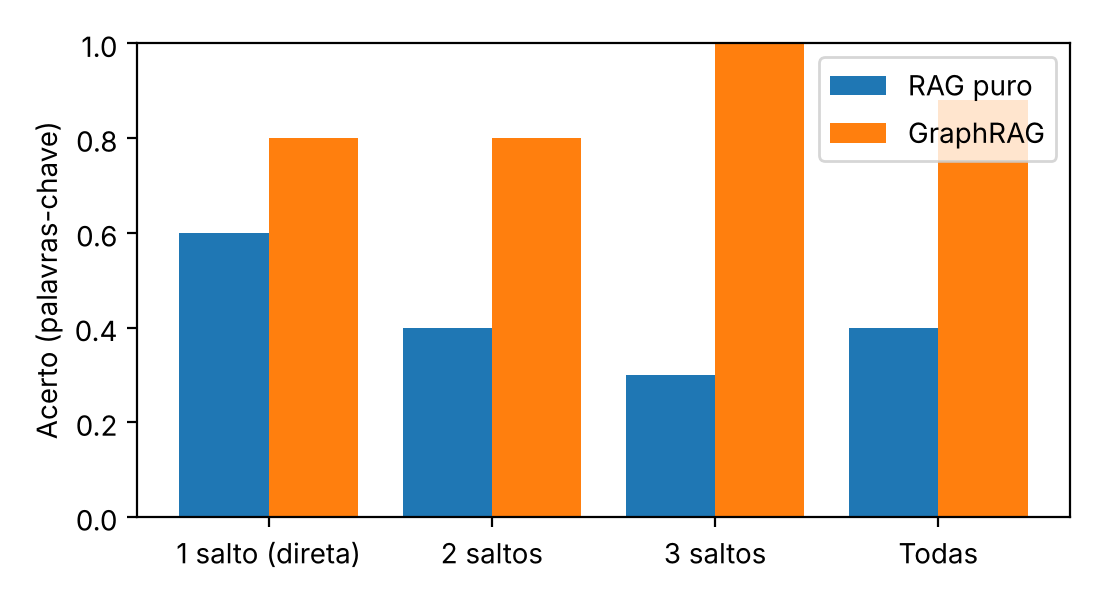
\includegraphics[width=0.7\linewidth]{fig_acerto.png}\caption{Acerto por faixa de saltos.}\end{figure}
\todo{Descrever onde o GraphRAG ganha e onde não ganha; a taxa de abstenção do RAG puro (17 de 30) pesa no acerto e precisa ser discutida.}
\subsection{Discussão}
\todo{Análise de erros: falhas de extração propagadas ao grafo; Cypher gerado incorretamente; armadilhas em que
a entidade existe mas o fato não.}

\section{Limitações e ameaças à validade} % [todos]
\todo{Grafo pequeno e esparso; erros de extração; juiz LLM pode ser enviesado; N pequeno (sem significância estatística);
gabarito derivado do próprio grafo favorece o GraphRAG --- discutir e mitigar.}

\section{Conclusão} % [D]
\todo{Resposta à pergunta de pesquisa com os números; trabalhos futuros.}

\section*{Contribuição de cada autor}
\todo{Se o professor exigir.}

\bibliographystyle{plain}
\bibliography{referencias}
\end{document}
